\chapter{Потоковые шифры}\label{chapter-stream-ciphers}
\selectlanguage{russian}

\section{Посимвольное шифрование}
\selectlanguage{russian}

Потоковые шифры осуществляют посимвольное шифрование открытого текста. Их основные достоинства: большая скорость шифрования по сравнению с блоковыми шифрами и относительно простая реализация.

Пусть имеется двоичная последовательность $x_{1} x_{2} \dots x_{N}$, представляющая открытый текст, и последовательность ключей $k_{1} k_{2} \dots k_{N}$. Шифрованная последовательность представляет собой сумму по модулю 2 этих двух последовательностей:
\[ \begin{array}{l}
    y_{1} = x_{1} \oplus k_{1}, \\
    y_{2} = x_{2} \oplus k_{2}, \\
    \dots \\
    y_{N} = x_{N} \oplus k_{N}.
\end{array} \]

Если бы в двоичной последовательности ключей все символы были независимы, и нули и единицы равновероятны, то такая система по доказанному выше была бы совершенной, то есть обеспечивала бы независимость шифрованного текста от исходного текста и, как следствие, равенство нулю количества взаимной информации. Поэтому одна из основных задач при разработке систем потокового шифрования состоит в построении последовательностей с равномерным, случайным и независимым распределением.

Существует много способов построения двоичных последовательностей с распределением, близким к равномерному. Они называются псевдослучайными последовательностями\index{число!псевдослучайное}.

Пусть имеем некоторую двоичную последовательность $z_{1} z_{2} \ldots z_{N}$, полученную в результате подбрасывания <<неправильной монеты>> (монета считается неправильной, так как даёт неравномерное распределение). Когда выпадал герб, записывали символ $1$. Когда выпадала решка, записывали символ $0$. Чтобы теперь приблизить распределение к равномерному, преобразуем эту последовательность с помощью алгоритма Джона фон Неймана (John von Neumann). Разделим символы на пары. Если $z_{1} z_{2} = 11$ или $z_{1} z_{2} = 00$, то пара выбрасывается из последовательности; если $z_{1} z_{2} =10$, то записываем новый символ $u=1$; если $z_{1} z_{2} =01$, то записываем новый символ $u=0$. Получаем новую двоичную последовательность символов $u_{1}u_{2}\ldots $, у которой распределение нулей и единиц ближе к равномерному.
%(См. \textbf{Приложение 2}).


\section{Криптостойкие последовательности}\label{chapter-crypto-random}

Генераторы псевдослучайных чисел (ГПСЧ) ставят в соответствие набору символов $z_{1} z_{2} \dots z_{l}$ значение некоторой функции $f(z_{1} z_{2} \dots z_{l}) = f_{1}$. Следующим $l$ символам -- $f(z_{l+1} z_{l+2} \dots z_{2l}) = f_{2}$. Получают набор значений $f_{1} f_{2} \dots f_{N}$ и используют их в качестве случайной последовательности.

Для проверки степени близости к независимости и равномерному распределению символов существует набор тестов. Американский институт стандартизации NIST разработал 16 тестов на псевдослучайность: подсчитывается число нулей и единиц, число одинаковых соседних пар, число одинаковых подпоследовательностей, автокорреляция, частота следующего символа в зависимости от предыдущих и т.~д. Вычисляют вероятность символа 0 (или 1)
\[
    P(f_i = 0 | f_{i-1} f_{i-2} \dots f_{i-k}) = \frac{1}{2} - \epsilon.
\]
Если вычисления осуществляются за полиномиальное время от длины подпоследовательности $k$, то есть с количеством битовых операций $O(k^{\textrm{const}})$, то тест называют \emph{полиномиальным}\index{задача!полиномиальная}.

Псевдослучайная последовательность удовлетворяет \emph{тесту <<следующего бита>>}, если не существует полиномиального по $k$ теста, позволяющего по предыдущим $k$ битам определить следующий бит с вероятностью, отличной от $\frac{1}{2} - \epsilon$, принимая во внимание погрешность оценки $\epsilon$. Последовательность, удовлетворяющая тесту <<следующего бита>>, также удовлетворяет всем возможным полиномиальным тестам по $k$ на равномерность распределения, и наоборот.

Последовательность называется \emph{криптографически стойкой} или \emph{криптостойкой}, если она удовлетворяет тесту <<следующего бита>>.

\subsection{Генератор BBS}
\selectlanguage{russian}

Имеются примеры <<хороших>> генераторов, вырабатывающих криптографически стойкие последовательности, например генератор Blum-Blum-Shub (BBS). Алгоритм работы состоит в следующем: выбирают большие (длиной не менее 512 бит) простые числа\index{число!простое} $p, q$, которые при делении на $4$ дают в остатке $3$. Вычисляют $n = p q$, с помощью генератора случайных чисел вырабатывают число $x_{0}$, где $1 \leq x_0 \leq n-1$ и $\gcd(x_0, n) = 1$. Далее проводят следующие вычисления:
\[ \begin{array}{l}
        x_{1} = x_{0}^{2} \mod n,\\
        x_{2} = x_{1}^{2} \mod n,\\
        \dots,\\
        x_{N} = x_{N-1}^{2} \mod n.
\end{array} \]

Для каждого вычисленного значения оставляют один младший разряд. Вычисляют двоичную псевдослучайную последовательность $k_1, k_2, k_3, \dots$ :
\[ \begin{array}{l}
        k_{1} = x_{1} \mod 2,\\
        k_{2} = x_{2} \mod 2,\\
        \dots,\\
        k_{N} = x_{N} \mod 2.
\end{array} \]

Число $a$ называется \emph{квадратичным вычетом} по модулю $n$, если для него существует квадратный корень $b$ (или два корня): $a = b^2 \mod n$. Для $p,q ~=~ 3 \mod 4$ верно утверждение, что квадратичный вычет имеет единственный корень, и операция $x \rightarrow x^2 \mod n$, применённая к элементам множества всех квадратичных вычетов $\set{QR}_n$ по модулю $n$, является перестановкой множества $\set{QR}_n$.

Полученная последовательность квадратичных вычетов $x_1, x_2, x_3, \dots$ -- периодическая с периодом $T < |\set{QR}_n|$. Чтобы её период для случайного $x_0$ с большой вероятностью оказался большим, числа $p,q$ выбирают с условием малого $\gcd(\varphi(p-1), \varphi(q-1))$, где $\varphi(n)$ -- функция Эйлера.

Полученная последовательность ключей является криптографически стойкой. Доказано, что для <<взлома>> (то есть определения следующего символа с вероятностью, большей $\frac{1}{2}$) требуется разложить число $n=pq$ на множители. Разложение числа на множители считается трудной задачей, все известные алгоритмы не являются полиномиальными по $\log_2 n$.

Оказывается, что если вместо одного последнего бита $k_i = x_i \mod 2$ брать $O(\log_2 \log_2 n)$ последних битов рассмотренного выше генератора $x_i$, то полученная последовательность останется криптостойкой.

Большим недостатком генератора BBS является малая скорость генерирования битов.


%\subsection{Генератор Микали}\index{генератор!Микали}

Другой пример -- генератор Микали.

Так же выбирают большие простые числа $p,q$ с битовой длиной не менее 512, вычисляют число $n = pq$. Находят функцию Эйлера $\varphi(n) = (p-1) (q-1)$ и задают целое число $e$ такое, что наибольший общий делитель $\gcd(e, \varphi(n)) = 1$. С помощью генератора случайных чисел выбирают $0 \leq x_{0} \leq n-1$. Вычисляют
\[ \begin{array}{l}
    x_1 = x_0^e \mod n, \\
    x_2 = x_1^e \mod n, \\
    \dots \\
    x_N = x_{N-1}^e \mod n.
\end{array} \]
Чтобы уменьшить сложность вычислений, в значениях $x_i$ оставляют $l$ младших разрядов, причём $l \leq \log_2 \log_2 N$. Последовательность ключей получают в виде
\[ \begin{array}{l}
    k_1 = x_1^2 \mod 2, \\
    k_2 = x_2^2 \mod 2, \\
    \dots \\
    k_N = x_N^2 \mod 2. \\
\end{array} \]

Как и генератор BBS, генератор Микали -- криптостойкий, для его взлома требуется разложить число $n$ на множители. Недостаток -- маленькая скорость.


\section{Последовательности максимального периода}
\selectlanguage{russian}
\label{section:max-seq}

Периодические последовательности с максимальным периодом называются $M$-последовательностями\index{$M$-последовательность} и характеризуются идеальной функцией автокорреляции.

Пусть $M$-последовательность имеет вид $x_1, x_2, \dots, x_n$, где значения $x_{i} = \pm 1$. Функция автокорреляции\index{функция!автокорреляции} такой последовательности имеет вид
\[
    \sum\limits_{i=1}^{T} x_i x_{i + \tau}  = \left\{ \begin{array}{l}
        -1, ~ \tau \neq 0, \\
        T, ~ \tau = 0. \\
    \end{array} \right.
\]

$M$-последовательности можно генерировать с помощью регистров сдвига с линейной обратной связью. На рис.~\ref{fig:impulse} показан регистр сдвига, состоящий из ячеек памяти со входами для информационных символов и тактовых импульсов. На рис.~\ref{fig:generator} тактовые импульсы опущены. Через $S_{j}$ обозначено содержимое $j$-й ячейки, где $j=\overline{0,L-1}$. В цепь обратной связи введены сумматоры по модулю 2 и умножители с коэффициентами $c_{j}$, принимающими значения $0,1$. Поступление тактового импульса вызывает сдвиг в регистре сдвига.
\begin{figure}[!ht]
	\centering
    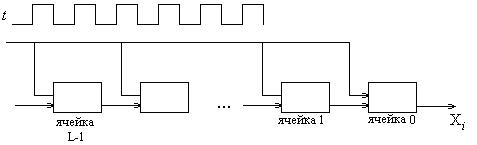
\includegraphics[width=0.8\textwidth]{pic/taktovi-impuls}
    \caption{Тактовые импульсы\label{fig:impulse}}
\end{figure}

В этой схеме используется линейная обратная связь. Выход ячейки с номером $L-1$ умножают на $c_{1}$, выход следующей ячейки $L-2$ умножают на $c_2$ и так далее. После умножения выходы ячеек суммируют по модулю 2 и результат подают на вход крайней ячейки $(L-1)$. Если содержимое всех ячеек состоит из нулей, то генерируемая последовательность также состоит из одних нулей. Если имеется ненулевое заполнение $S_{j-1}, S_{j-2}, \dots, S_{j-L}$, то после поступления $j$-го тактового импульса имеем сигнал на выходе такой, как показано на рис.~\ref{fig:generator}:
\begin{figure}[!ht]
	\centering
	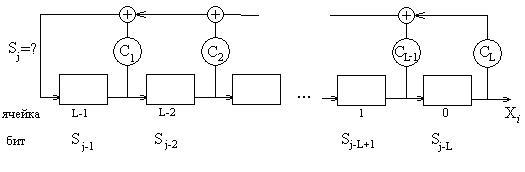
\includegraphics[width=0.8\textwidth]{pic/generator}
    \caption{Генератор\label{fig:generator}}
\end{figure}

Во всем разделе~\ref{section:max-seq}  операцией <<$+$>>  обозначается операция сложения двоичных коэффициентов и многочленов по модулю 2.
\[
    S_{j} = c_{1} S_{j-1} + c_{2} S_{j-2} +  \dots  + c_{L-1} S_{j-L+1} + c_{L} S_{j-L}.
\]

Это соотношение определяет принцип работы генератора на регистрах сдвига\index{регистр сдвига}. Всего $2^{L}$ начальных условий, задающих значения бит в ячейках, из них $2^{L}-1$ ненулевых начальных условий. Генерируемая двоичная последовательность является периодической с периодом $T\leq 2^{L}-1$. Величина периода зависит от коэффициентов обратной связи $c_{1},  \ldots, c_{L} $.

Набор коэффициентов задаётся многочленом обратной связи
    \[ c(y) = 1 + c_1 y+ c_2 y^2 + \dots + c_L y^L. \]
Свойства этого многочлена влияют на период генерируемой последовательности. Рассмотрим его подробнее.

Многочлен $c(y)$ над полем $\GF{2}$ с коэффициентами $c_i \in \GF{2}$ называется \textit{приводимым}, если его можно представить в виде произведения многочленов меньшей степени. Например, многочлен $1 + y^{2} = (1 + y) (1 + y) = 1 + y + y + y^2 = 1 + y^2$ является приводимым. Многочлен $1 + y + y^{2}$ -- неприводимый.

Приведем без доказательства два важных утверждения.
\begin{itemize}
    \item Пусть $c(y)$ -- неприводимый многочлен. Тогда существует такое значение $m$, что $y^{m} + 1$ делится без остатка на $c(y)$, то есть $\frac{y^{m} + 1}{c(y)} = d(y)$.
    \item Существуют многочлены $c(y)$, для которых $m=2^{L} - 1$, где L -- степень многочлена $c(y)$. Эти многочлены называются примитивными.
\end{itemize}

Если $c(y)$ -- примитивный многочлен\index{многочлен!примитивный}, то период генерируемой последовательности является максимальным, то есть равным $T = 2^{L} - 1$. Генерируемые последовательности являются $M$-последовательностями, то есть последовательностями максимального периода. Для любого начального ненулевого состояния генерируется циклический сдвиг одной и той же последовательности максимального периода $T=2^{L} - 1$.

Оказывается, что многочлен обратной связи и состояние регистра определяются однозначно по $2L$ последовательным символам выхода регистра сдвига с линейной обратной связью (с помощью алгоритма Берлекэмпа~---~Мэсси или алгоритма Евклида).

Например, в спутниках GPS имеется регистр сдвига c 43 ячейками и периодом генерируемой последовательности $2^{43} - 1$. Длительность одного импульса $\sim 0{,}1$ мкс, период последовательности примерно равен одному году. Если бы для генерирования криптостойкой последовательности был просто применён регистр сдвига с линейной обратной связью, то, чтобы найти многочлен обратной связи, криптоаналитику достаточно было бы получить 86 символов последовательности.

Чтобы РСЛОС можно было использовать в качестве составной части криптографически стойкого генератора псевдослучайной последовательности или поточного шифра, создатели криптографических примитивов комбинируют несколько регистров сдвига, в том числе с помощью приводимых далее способов.


\section[Три способа улучшения последовательностей]{Три способа улучшения \protect\\ последовательностей}

\subsection[Генераторы с несколькими регистрами сдвига]{Генераторы с несколькими регистрами \protect\\ сдвига}
\selectlanguage{russian}

Первый способ улучшения криптографических свойств последовательности состоит в создании композиционных генераторов из нескольких регистров сдвига при определённом способе выбора параметров. Схема такого генератора показана на рис.~\ref{fig:generators}. Здесь $L_i, ~ i = 1, 2, \dots, M$ -- регистры сдвига с линейной обратной связью. Вырабатываемые ими двоичные символы $x_{1,i}, x_{2,i},  \dots, x_{M,i}$ поступают синхронно на устройство преобразования, задаваемое булевой функцией $f(x_{1,i}, x_{2,i}, \dots, x_{M,i})$. В булевой функции аргументы принимают значения $0,1$ и значения функции также $0,1$.

Число ячеек в $i$-м регистре равно $L_{i}$, причём $\gcd(L_i, L_j)=1$ для $i \neq j$, где $\gcd$ -- наибольший общий делитель. Общее число ячеек $L = \sum\limits_{i=1}^M L_i$. Булева функция $f$ должна включать слагаемое по одному из входов, т.~е. $f = \dots + x_i + \dots$, для того чтобы двоичные символы на выходе этой функции были равновероятными. Период этого генератора может достигать величины (немного меньше)
    \[ T \simeq 2^L. \]

\begin{figure}[!ht]
	\centering
	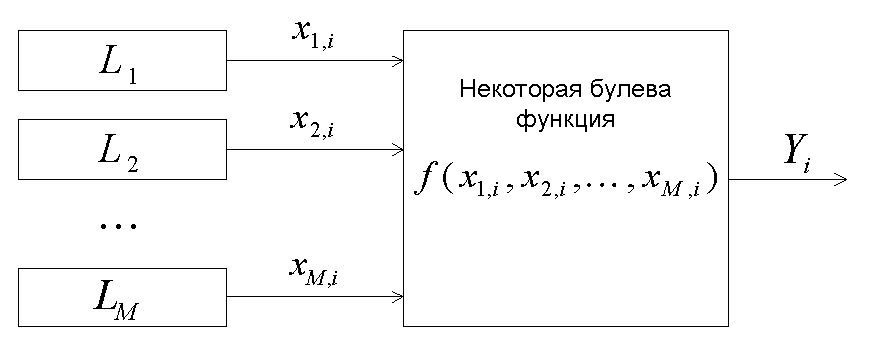
\includegraphics[width=0.7\textwidth]{pic/generators}
    \caption{Генератор с несколькими регистрами сдвига\label{fig:generators}}
\end{figure}

Таким образом, увеличение числа регистров сдвига с обратной связью увеличивает период последовательности. Однако более важным параметром для увеличения криптостойкости генератора является \emph{ длина регистра с линейной обратной связью}, эквивалентного по порождаемой последовательности. Такой эквивалентный регистр с линейной обратной связью находится с помощью алгоритма Берлекэмпа~---~Мэсси декодирования циклических кодов. В лучшем случае длина эквивалентного регистра соизмерима с периодом последовательности, порождённой нелинейным генератором. В общем случае определение эквивалентной длины является сложной задачей.


\subsection[Генераторы с нелинейными преобразованиями]{Генераторы с нелинейными \protect\\ преобразованиями}
\selectlanguage{russian}

Известно, что любая булева функция $f(x_1, x_2, \dots, x_M)$ может быть единственным образом записана многочленом Жегалкина\index{многочлен!Жегалкина}:
\[ \begin{array}{ll}
    f(x_1, x_2, \dots, x_M) & = ~c~ \oplus \\
    & \oplus \sum\limits_{1 \leq i \leq M} c_i x_i \oplus \\
    & \oplus \sum\limits_{1 \leq i < j \leq M} c_{i,j} x_i x_j \oplus \\
    & \oplus \sum\limits_{1 \leq i < j < k \leq M} c_{i,j,k} x_i x_j x_k \oplus \\
    & \oplus \dots \oplus \\
    & \oplus ~ c_{1,2,\dots,M} ~ x_1 x_2 \dots x_M.
\end{array} \]

%Криптографу рекомендуется выбирать булеву функцию с возможно большим числом ненулевых коэффициентов при квадратичных членах полинома Жегалкина.

Второй способ улучшения криптостойкости последовательности поясняется с помощью рис.~\ref{fig:lfsr-zhegalkin}, на котором представлен регистр сдвига с $M$ ячейками и устройство, осуществляющее преобразование с помощью булевой функции $f(x_1, x_2, \dots, x_M)$, причём функция $f$ содержит нелинейные члены, то есть произведения $x_i x_j \dots$. Тактовый вход здесь такой же, как у регистров, показанных на других рисунках.

Если функция $f$ нелинейная, то в общем случае неизвестен полиномиальный алгоритм восстановления состояния регистров по нескольким последним выходам генератора. Таким образом, использование нескольких регистров сдвига увеличивает максимально возможный период по сравнению с одним регистром до $T < 2^{L_1 + L_2 + \dots + L_M}$, а нелинейность функции $f$ позволяет избежать простого нахождения состояния по выходу. Чтобы улучшить криптостойкость последовательности, порождаемой регистром, рекомендуется брать много нелинейных членов многочлена Жегалкина.

Такой подход применён в системе GPS. Удачных попыток её взлома до сих пор нет.

\begin{figure}[!ht]
    \centering
	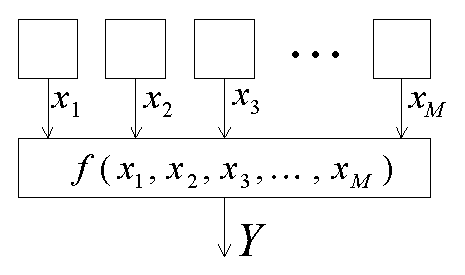
\includegraphics[width=0.4\textwidth]{pic/lfsr-zhegalkin}
    \caption{Криптографический генератор с нелинейной булевой функцией\label{fig:lfsr-zhegalkin}}
\end{figure}


\subsection[Мажоритарные генераторы, шифр A5/1]{Мажоритарные генераторы на примере алгоритма шифрования A5/1}\label{section:majority_generators}\index{шифр!A5}
\selectlanguage{russian}

Третий способ улучшения криптостойкости последовательностей поясняется с помощью рис.~\ref{fig:gsm-a51-cipher}, на котором показан мажоритарный генератор ключей алгоритма потокового шифрования A5/1 стандарта GSM. В отличие от случая нелинейного комбинирования выходов нескольких регистров в этом случае применён условный сдвиг регистров, то есть на каждом такте некоторые регистры могут не сдвигаться, а оставаться в прежнем состоянии. На рисунке показана схема из трёх регистров сдвига с различными многочленами обратной связи (здесь применена обратная нумерация ячеек, коэффициентов и переменных по сравнению с предыдущими разделами):
\[ \left\{ \begin{array}{l}
    c_1(y) = y^{19} + y^{18} + y^{17} + y^{14} + 1, \\
    c_2(y) = y^{22} + y^{21} + 1, \\
    c_3(y) = y^{23} + y^{22} + y^{21} + y^8 + 1.
\end{array} \right. \]

\begin{figure}[!ht]
    \centering
	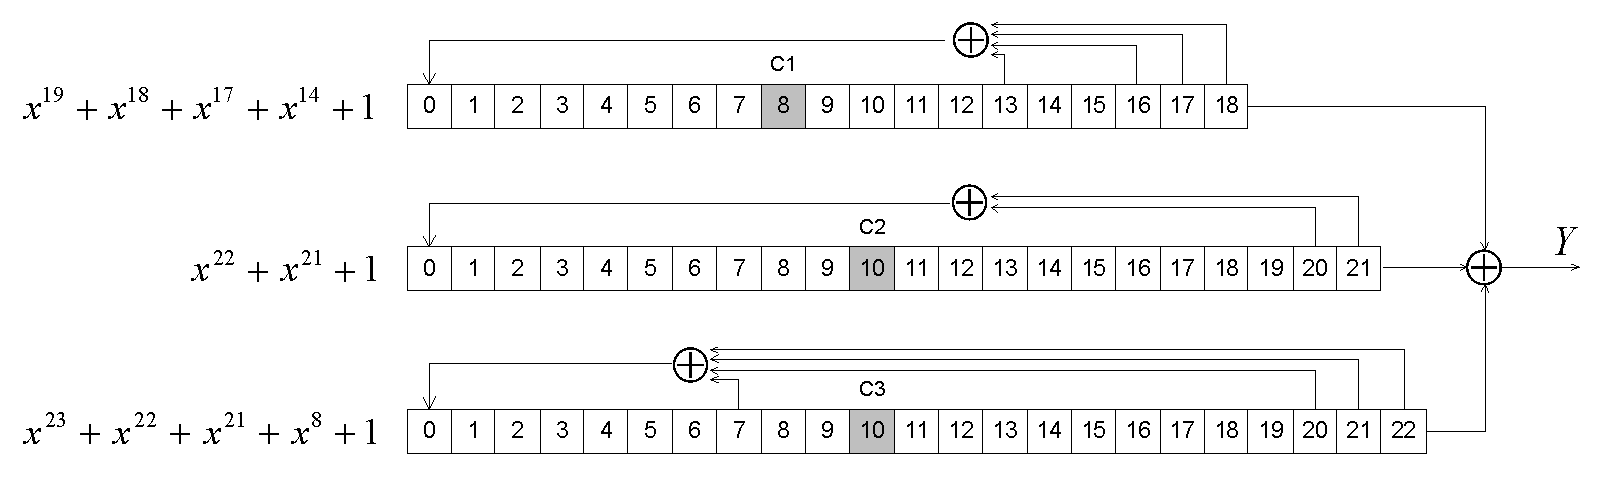
\includegraphics[width=\textwidth]{pic/gsm-a51-cipher}
    \caption{Регистр сдвига алгоритма шифрования A5/1\label{fig:gsm-a51-cipher}}
\end{figure}

В алгоритме A5/1 регистры сдвигаются не на каждом такте. Правило сдвига следующее. В каждом регистре есть один тактовый бит, определяющий сдвиг, -- восьмой бит $\textrm{C1}$ для первого регистра, десятые биты $\textrm{C2}$ и $\textrm{C3}$ для второго и третьего регистров. На каждом такте вычисляется мажоритарное значение тактового бита $m = \textrm{majority}(\textrm{C1}, \textrm{C2}, \textrm{C3})$, то есть по большинству значений: 0 или 1. Если для данного регистра значение тактового бита совпадает с мажоритарным решением, то регистр сдвигается. Если не совпадает, то остаётся в прежнем состоянии без сдвига на следующий такт. Так как всего состояний тактовых битов $2^3$, то в среднем каждый регистр сдвигается в $\frac{3}{4}$ всех тактов.

Общее количество ячеек всех трёх регистров $19+22+23=64$, следовательно, период генератора A5/1: $T < 2^{64}$. Данный шифр не может считаться стойким из-за возможности полного перебора. Например, известны атаки на шифр A5/1, требующие 150-300 GiB оперативной памяти и нескольких минут вычислений одного ПК (2001 г.).

